\paragraph{Learning procedure, policy network, and hyper-parameters.}
Each state representation requires a different neural net for the policy network.
%
For \textbf{HF}, we use a $3$-layer fully connected network. Before training, we run the
pipeline with a random policy $100$ times to calculate the mean and standard
deviation of each feature, and use this metadata to normalize all features into
mean of $0$ deviation of $1$.

For \textbf{IV}, we run the \emph{caller}, the \emph{callee}, the \emph{calling context}
and the \emph{arguments bitvector} through four separate $2$-layer
GRU~\cite{gru} blocks, concatenate the last hidden outputs of these $4$ blocks,
and then feed it to a $3$-layer fully connected network. The architecture is
depicted in Fig.~\ref{fig:inst2vec_occam}.

Both networks use ReLU~\cite{relu} as the activation function. 
% Ashish: Should a citation be added for ReLU above?
We use \reinforce~\cite{reinforce} with normalized rewards to update
the policy for both models. At each \reinforce iteration, we roll out
$k$~runs of the current policy, batch them together, and use the Adam
optimizer~\cite{adam} to update the network. For all metrics, we use the same
hyper-parameters: \insttovec calling
context $n = 10$, number of runs in each policy rollout $k =75$, Adam's learning rate = $0.001$, and train up to $340$ iterations.

     \begin{figure}
         \centering
         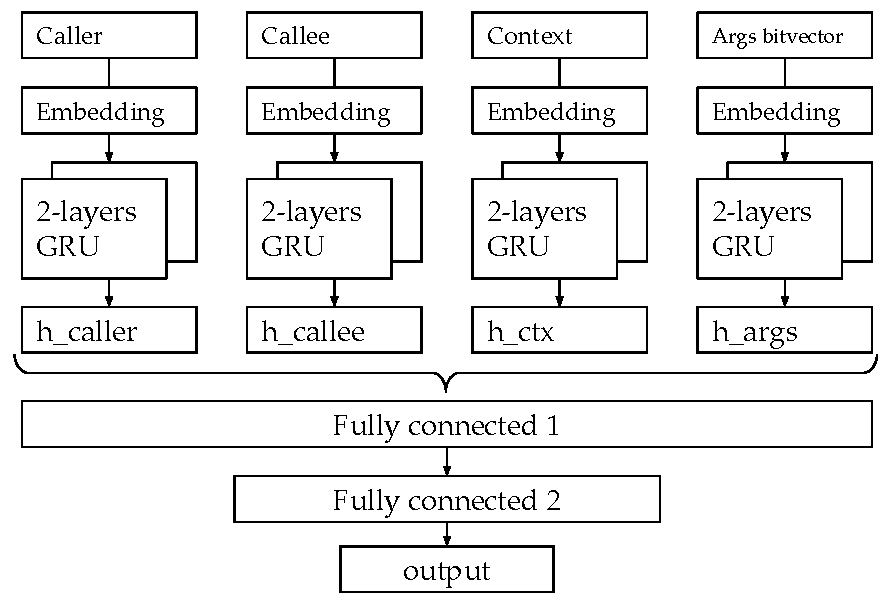
\includegraphics[width=0.75\textwidth]{doccam_figures/inst2vec_occam.pdf}
         \caption{Policy network architecture using \insttovec .}
         \label{fig:inst2vec_occam}
     \end{figure}
     \begin{figure}
         \centering
         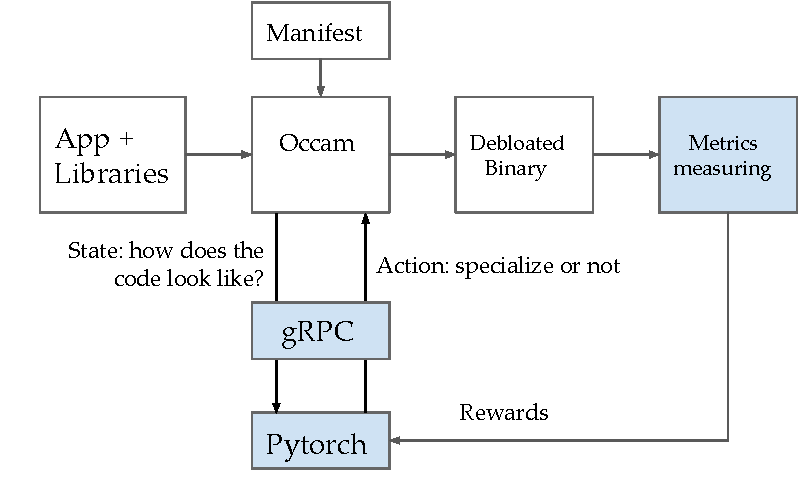
\includegraphics[width=0.75\textwidth]{doccam_figures/D-OCCAM.pdf}
         \caption{\doccam architecture. Boxes in blue correspond to this work.}
         \label{fig:d-occam}
     \end{figure}


%%% Local Variables:
%%% mode: latex
%%% TeX-master: "neurips_2019"
%%% End:
